\section{On the Edge Computing}

As opposed to conventional visual monitoring systems (CCTVs, IP cameras), that send the video data to a data center to be stored and processed, embedded smart cameras process the image data directly on board. 
In this proposal we present:

\begin{itemize}[noitemsep] % [noitemsep] removes whitespace between the items for a compact look
\item \textit{Our aproach} to on-board smart camera computing.
\item \textit{Hardware and Software description}.
\item \textit{Actual real Use Case implementation} of our product. 
\end{itemize}


 Nevertheless, there is strong demand for mobile vision solutions ranging from object recoginiotn to advanced human-machine interfaces.

\subsection{Our Aproach}

The problem of on-board computing and further analysis of live video feed is an ongoing research. We follow the next procedure which is focused on 3 main cicles which are:

\begin{figure}[H]\centering
	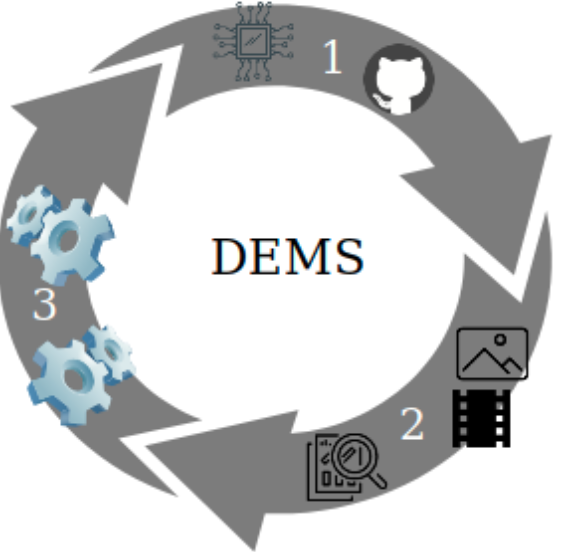
\includegraphics[width=\linewidth]{images/cicle}
	\caption{Cicle of work}
	\label{fig:cicle}
\end{figure}

% Explain the DEMS cicle for target project
\begin{itemize}

\item[1] \textit{Algorithm Design}. If the client requirement does not have precedents, we partially hand craft a Computer Vision Algorithm applied to client use case for further data recolection, analysis and improves.
\item[2] Data Analysis for client use cases and presentation of results according to initial requierements.
\item[3] \textit{Improvement}. Improve original algorithm using the  propietary collected data with the use of Machine Learning techniques (if is requiered also with hardware udgrade).
     
\end{itemize}

We dedicate a specialized team to solve the problems in each cycle. The case study that we present in the whole proposal, complete 2 of the 3 states of our cicle of work, and we are currently working on an improvement of our main hardware and algorithm to provide greater security to our clients and at the same time increase our technology. Also be in an advantageous position above the competition thanks to the collected propietary data in order to create new products and improve existing ones.



\subsection{Hardware and Software description}
Below is a description of the hardware and software we use.

\subsubsection{Software Description}
If the requirements are very specific and no historic data is aviable, we design a algorithm with tradicional computer vision techniques according to the use case with focus on the embedding side; we maintain a constant monitoring of the program for the event that client is looking for and at the same time we collect data for three main purposes, improve the current algorithm with Machine Learning techniques, bring data for further applications by the side of client and by own, be propietary of labeled data in the target area of work.

Our main tools for the creation of custom algorithms are Python and C++ as main languages. OpenCV is our compendium of multiple purpose Computer Vision techniques which are used to hand craft the desired behavior of the program and data recollection.

\subsubsection{Hardware Description}

The figure 5 shows the main aspects of our smart-camera, this contains:
\begin{itemize}
\item[•] A Low resolution camera which is used for detection of flow in the video
\item[•] A HD 8MP camera is used for capture the main aspects of interest when the Low resolution camera trigers the signal of capture. 
\item[•] We also develop a optional pripietary Integrated Circuit with the main idea of triger the infra-red filter for the HD camera. Also this can be used for further sensor integrations, by now we are using it also as a GPS tracker for the device. 
\end{itemize} 

\begin{figure}[H]\centering
	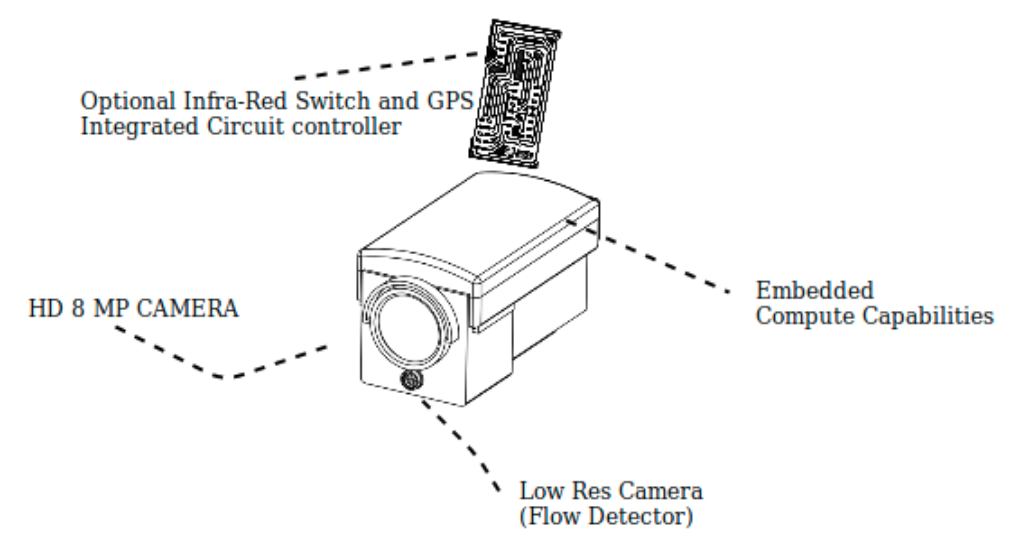
\includegraphics[width=\linewidth]{images/hardware_desc}
	\caption{Schematics of our hardware}
	\label{fig:hardware_dec}
\end{figure}

The compute capabilities of our enveded device are descrived below:

\begin{itemize}[noitemsep]

\item[•] SoC: Broadcom BCM2837B0 quad-core A53 (ARMv8) 64-bit @ 1.4GHz
\item[•] GPU: Broadcom Videocore-IV 256 MB VRAM
\item[•] RAM: 1GB LPDDR2 SDRAM
\item[•] Networking: Gigabit Ethernet (via USB channel), 2.4GHz and 5GHz 
\item[•] 802.11b/g/n/ac Wi-Fi
\item[•] Bluetooth: Bluetooth 4.2, Bluetooth Low Energy (BLE)
\item[•] Storage: Micro-SD
\item[•] GPIO: 40-pin GPIO header, populated
\item[•] Ports: HDMI, 3.5mm analogue audio-video jack, 4x USB 2.0, Ethernet
\item[•] Camera Serial Interface (CSI), Display Serial Interface (DSI)
\item[•] Dimensions: 82mm x 56mm x 19.5mm, 50g
\item[•] Optional - Neural Network Compute Capabilities according to use case.
\end{itemize}


\subsection{Actual real Use Case implementation}

Below is a schematics of our embedded device working in the wild.

\begin{figure}[H]\centering
	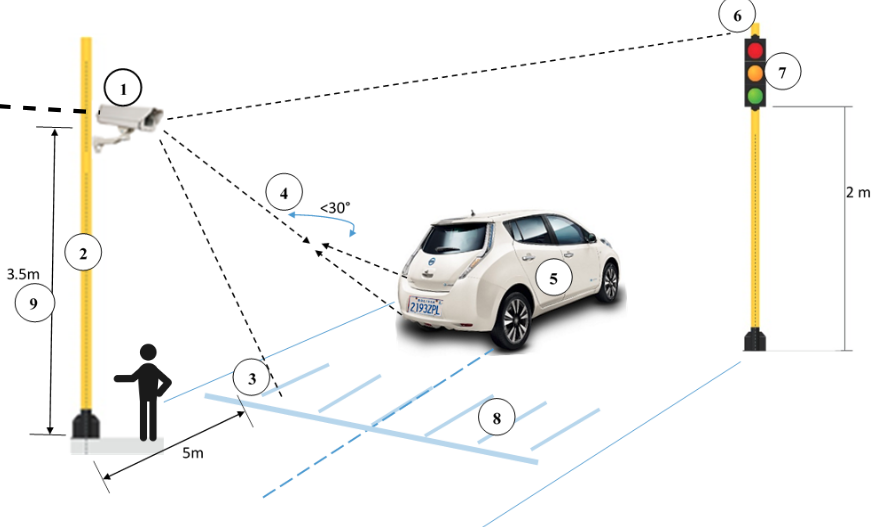
\includegraphics[width=\linewidth]{images/lucam}
	\caption{Actual use case of our embedded camera }
	\label{fig:work_dec}
\end{figure}

\begin{itemize}[noitemsep] % [noitemsep] removes whitespace between the items for a

\item[1]- On Board Computation according client requirement,this communicates his events to private cloud if internet access is aviable.
\item[2]- Mounting pole. The height to our device from ground, influence the algorithm behavior. 
\item[3-8]- Pedestrian crossing limit right/left side way.
\item[4]- Optimal vision angle for plate detection.
\item[5]- Target object, in this case cars
\item[6]- Traffic Light mounting pole,
\item[7]- Actual Traffic Light, the camera color sensor implemented by software sees the color transitions and control the algorithm behavior and cameras syncronization, as Figure 3 shows, Figure 3 shows the extract of 5 seconds video from Low resolution camera and a picture of High Resolution for target object with region of interest, this two assets, video and picture is the output of our custom algorithm.
\end{itemize}

As mentioned before, if you have an Internet connection, we can, in real time, make a wingspan of the information of video/picture and serve it to different users as required, or save it in a bucket for further analysis, the next diagram shows what it follows if we are online.


\begin{figure}[H]\centering
	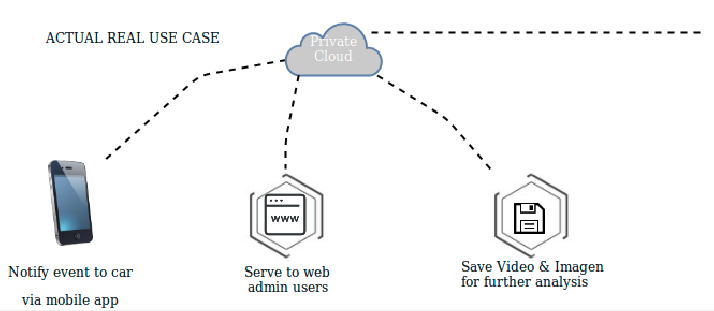
\includegraphics[width=\linewidth]{images/online}
	\caption{Online process for the information detected in the road. }
	\label{fig:work_dec}
\end{figure}

At the time of writing this, we are training a NN Algorithm to support the Hand Crafted algorithm  with the information of video and image generated from the beginning of this year 2018. Following our cicle of work of Figure 4, we generate enought labeled data for our use case and we are ready to start a new cicle of production.

You can see the partial results of this project in our test page \href{www.demsbo.com}{www.demsbo.com} and our github project \href{https://github.com/alvarohurtadobo/prototipo}{https://github.com/alvarohurtadobo/prototipo}.

